\documentclass[11pt,a4paper]{article}

\usepackage[a4paper,top=1.75cm,bottom=1.75cm,left=1.95cm,right=1.95cm]{geometry}
\usepackage[T1]{fontenc}
\usepackage{lmodern}
\usepackage{setspace}
\usepackage{booktabs}
\usepackage{graphicx}
\usepackage{amsmath,amssymb}
\usepackage[numbers,sort&compress]{natbib}
\usepackage[hidelinks]{hyperref}
\usepackage{microtype}

\onehalfspacing
\setlength{\parskip}{0.16em}
\setlength{\textfloatsep}{6pt plus 2pt minus 2pt}
\setlength{\intextsep}{6pt plus 2pt minus 2pt}
\setlength{\abovecaptionskip}{3pt}
\setlength{\belowcaptionskip}{2pt}
\renewcommand{\topfraction}{0.90}
\renewcommand{\bottomfraction}{0.85}
\renewcommand{\textfraction}{0.08}
\renewcommand{\floatpagefraction}{0.82}

\begin{document}

% =========================================================================
% COVER PAGE (Excluded from CS482 3-5 A4 Page Main Text Limit)
% =========================================================================
\pagenumbering{roman}
\begin{titlepage}
\centering
\vspace*{1.2cm}
{\large CS482 Data Science --- Group Project (Phase A Draft)\par}
\vspace{0.8cm}
{\LARGE\bfseries Corporate Event Shocks, Realized Volatility, and Downside
Tail-Risk Forecasting in U.S.\ Equities (2019--2025)\par}
\vspace{0.4cm}
{\large Econometric Panel HAR-RV, Per-Stock GJR-GARCH(1,1), Calibrated
LightGBM, and Train-Background TreeSHAP Under Leakage-Free Purged Splits\par}
\vspace{1.2cm}

{\small
\begin{tabular}{ll}
\toprule
\textbf{Group Member \& Role} & \textbf{Student ID (Replace Before Moodle)} \\
\midrule
Member A (Financial Data \& Freeze) & [Student ID A] \\
Member B (Panel Econometrics \& GARCH) & [Student ID B] \\
Member C (LightGBM, Calibration \& TreeSHAP) & [Student ID C] \\
Member D / All (Phase B QLoRA \& Audit) & [Student ID D] \\
\bottomrule
\end{tabular}
}

\vspace{1.0cm}
\begin{minipage}{0.88\textwidth}
\small\raggedright
\textbf{Academic Research \& Non-Investment-Advice Notice.}
This study is conducted solely for CS482 academic coursework and methodological
evaluation of associational and predictive risk models (academic research only;
\textbf{not investment advice}). It makes no causal claims and does not
constitute investment, financial, or trading advice. All empirical statistics
are generated programmatically from the frozen Phase A bundle
(\texttt{panel\_daily.parquet} SHA-256 prefix \texttt{3515fcd12cab}).
\end{minipage}

\vfill
{\normalsize Phase A Freeze Date: November 2026 \quad | \quad
Target Final Submission: December 14, 2026\par}
\end{titlepage}

% =========================================================================
% MAIN TEXT (CS482 Requirement: 3-5 A4 Pages, Single-Column, 11pt, 1.5 Spacing)
% =========================================================================
\pagenumbering{arabic}
\setcounter{page}{1}

\section{Introduction, Research Question, and Hypotheses}

Forecasting short-horizon equity volatility and downside tail-risk episodes
matters directly to portfolio risk managers, volatility-targeting allocators,
and financial stability researchers because market turbulence clusters across
regimes while return levels closely resemble a random walk. Rather than
forecasting noisy directional prices, this study examines 5-day forward realized
volatility and downside tail-risk events across a deterministic cross-sector
universe of 60 liquid U.S.\ equities over 2019--2025, spanning the
2020 COVID-19 shock, the 2022 monetary tightening bear market, the 2024
expansion, and 2025 AI and policy volatility.

\textbf{Research Question.} Under strict purged and embargoed chronological
splits, how reliably do classical econometric baselines (panel HAR-RV and
per-stock GJR-GARCH(1,1)) and nonlinear gradient-boosted trees (LightGBM)
forecast 5-day forward annualized realized volatility and downside tail-risk
events (5-day return $< -5\%$), and how strongly are lagged negative returns and
implied volatility (VIX) associated with future volatility across sectors? We
pre-register three falsifiable hypotheses:
\begin{itemize}\setlength{\itemsep}{0pt}\setlength{\parsep}{0pt}
\item \textbf{H1 (Confirmatory, Associational):} Lagged negative daily returns
(leverage association) and lagged VIX are positively associated with forward
5-day log realized volatility, with heterogeneity across growth/cyclical and
defensive sectors.
\item \textbf{H2 (Confirmatory, Predictive):} Under quarterly expanding purged
backtesting, global LightGBM outperforms Persistence, per-stock GJR-GARCH(1,1),
and Panel HAR-RV on 2025 holdout QLIKE/RMSE and downside tail-risk PR-AUC, while
2024 validation calibration improves probability reliability (ECE).
\item \textbf{H3 (Deferred to Phase B):} Event-anchored 4-bit QLoRA
fine-tuning of 27B--32B open LLMs on frozen pre-close SEC EDGAR event text adds
incremental 2025 tail-risk lift over price-only Phase A baselines (null results
accepted).
\end{itemize}
All Phase A conclusions are strictly associational or predictive and are not
investment advice.

\section{Data Collection, Leakage-Free Alignment, and Frozen Splits}

\textbf{Cross-Sector Universe and Market Data.} We fix a pre-2019
deterministic universe of 60 S\&P 500 bellwethers (12 stocks across
each of five GICS sectors: Technology, Financials, Healthcare, Consumer, and
Energy; zero 2025 lookahead). Daily split-adjusted OHLCV and dividend-adjusted
closes for all 60 equities plus \texttt{SPY} and
\texttt{\^{}VIX} are collected from Yahoo Finance across 1,760
canonical NYSE trading days (2019-01-02 to 2025-12-31; 105,600
stock-days, zero missing cells or zero-volume halts). Macro indicators from FRED
(\texttt{VIXCLS} and 10Y--2Y yield spread \texttt{T10Y2Y}) are aligned onto
the NYSE calendar using backward-only forward-fill (never backfilled), flagging
13 U.S.\ bond-market holidays.

\textbf{Authoritative Corporate Event Backbone.} Day-1 probes confirmed that
Hugging Face's \texttt{financial-news-multisource} is gated (HTTP 401 without
token) and lacks continuous 2024 intraday coverage, whereas \texttt{FNSPID}
terminates in 2023 and exhibits \texttt{00:00:00 UTC} timestamp leakage.
Following our pre-registered fallback, we ingest public SEC EDGAR Form
\texttt{8-K}, \texttt{8-K/A}, \texttt{10-Q}, and \texttt{10-K} filings
across 2019--2025, resolving holding-company predecessor CIKs for \texttt{BLK}
and \texttt{XOM} and recursively paginating 195 historical
\texttt{filings.files} archives to recover 7,703 unique
filings with 60/60 dual-period continuity (2024--2025 vs.\ 2019--2023 event-day
rate ratio 0.8860). All second-precision UTC
\texttt{acceptanceDateTime} stamps are converted to \texttt{America/New\_York}
(DST-aware): filings before 16:00 ET (13:00 ET on 15 scheduled NYSE early-close
half-days, shifting 2 post-13:00 \texttt{WFC} filings
to $t+1$) stay on day $t$, while post-close and holiday filings roll to $t+1$.
Intra-day headline deduplication removes 29 duplicates and
caps counts at $\le 5$/day, yielding 6,822 event-anchored
stock-days frozen for Phase B.

\textbf{Targets, Predictors, and Purged Splits.} Primary continuous target
\texttt{rv\_5d\_fwd} is the 5-day forward annualized Parkinson high-low range
volatility~\cite{parkinson1980} over $t+1\dots t+5$, modeled on
$y = \ln(\text{RV} + 10^{-6})$ with close-to-close sensitivity
\texttt{rv\_5d\_cc\_fwd}. Primary binary target \texttt{y\_tail} equals 1
iff 5-day forward cumulative adjusted return is below $-5\%$ (sensitivity
\texttt{y\_tail\_rv90} uses the Train-only 90th-percentile RV threshold
0.3742). All 22 predictors use strictly $\le t$ information.
Following \citet{lopezdeprado2018}, chronological splits enforce 6-trading-day
embargoes ($\ge h=5$): Train 2019-01-02 to 2023-12-20 (73,860
modeling rows after 21-day \texttt{rv\_m} warmup), Val 2024-01-02 to
2024-12-20 (14,760 rows, tuning/calibration only), and single-shot
Holdout Test 2025-01-02 to 2025-12-31 (14,700 scorable rows across
245 days; final 5 incomplete days masked \texttt{NA}). All frozen
artifacts are sealed under SHA-256 (\texttt{panel\_daily.parquet} prefix
\texttt{3515fcd12cab}).

\section{Econometric and Machine Learning Methodology}

\textbf{EDA and H1 Panel HAR-RV.} Cross-cycle EDA audits regime volatility,
leverage asymmetry, and tail-risk incidence across Train-median VIX regimes
($\text{VIX} \ge 19.61$). To test H1 across all 104,040
modeling-complete stock-days without pretest switching, we estimate a
within-entity Stock-FE extended Panel HAR-RV model~\cite{corsi2009}
interacting lagged negative returns ($\min(r_{i,t}, 0)$) and VIX with sector
indicators (Healthcare reference), using Bartlett-kernel Driscoll--Kraay
standard errors~\cite{driscoll1998} ($L=7$) to account for both
serial overlap and contemporaneous cross-stock shocks, with step-down
Holm--Bonferroni correction~\cite{holm1979} across the 5-test confirmatory
family and pre-specified Train-only, close-to-close, and entity-clustered
Newey--West sensitivities.

\textbf{H2 Out-of-Sample Forecasting, Calibration, and TreeSHAP.} Four models
share an identical quarterly expanding-window purged schedule (2024 Val, then
2025 Q1--Q4 with $\ge 5$ trading-day purge before every quarter): (i)
Persistence (\texttt{rv\_w} and expanding base rate); (ii) per-stock
GJR-GARCH(1,1)~\cite{glosten1993} on $100r_{i,t}$ with causal post-fit
variance filtering (300/300 fits converged); (iii) Stock-FE Predictive
HAR-RV back-transformed via fit-fold Duan smearing~\cite{duan1983} plus
Logistic HAR-RV; and (iv) Global LightGBM~\cite{ke2017lightgbm} tuned strictly
on 2024 Val QLIKE (regression) and PR-AUC (classification). To avoid in-sample
calibration overfitting, we compare Isotonic, Platt sigmoid, and 1-parameter
Temperature Scaling~\cite{guo2017calibration} via 4-quarter out-of-fold CV
strictly inside 2024 Val, selecting \texttt{isotonic}, refitting on
full 2024 Val, and freezing it for single-shot 2025 Test evaluation. Regression
is evaluated by variance-scale QLIKE~\cite{patton2011}, RMSE, and MAE;
classification by PR-AUC (primary), ROC-AUC, Brier, and 10-bin ECE, with 5-day
date-block bootstrap 95\% CIs ($B=1{,}000$) and $h=5$ Bartlett-PSD HLN-modified
Diebold--Mariano tests~\cite{harvey1997} (Holm-adjusted). Exact interventional
TreeSHAP~\cite{lundberg2020treeshap} uses a 1,000-row 2019--2023
Train background to audit LightGBM model behavior strictly non-causally.

\section{Empirical Results}

\textbf{Cross-Cycle Regimes and H1 Panel Evidence.} Mean 5-day annualized
Parkinson RV peaked during the 2020 COVID shock (0.3241) and 2022
bear market (0.2687), compressed in 2024 (0.1998), and
re-expanded in 2025 (0.2411; Figure~\ref{fig:regimes_forecasts}A--B).
In H1 (Table~\ref{tab:main_summary}, Panel A; Within $R^2 = 0.4736$),
overall 5-sector average leverage (-1.4458, Holm $p < 0.0001$;
negative slope on $\min(r_t,0)$ implies higher forward volatility after drops),
overall VIX (+0.0141, Holm $p < 0.0001$), and the joint 5-sector
interaction Wald test ($\chi^2 = 84.84$, Holm $p < 0.0001$) are
overwhelmingly significant across all sensitivities. However, pairwise
Technology vs.\ Healthcare interactions are not individually significant under
conservative Driscoll--Kraay SEs and Holm adjustment (leverage Holm
$p = 0.171$), whereas Financials and Energy exhibit the
strongest cyclical differentials relative to Healthcare. H1 therefore receives
partial, nuanced support.

\begin{figure}[!tb]
\centering
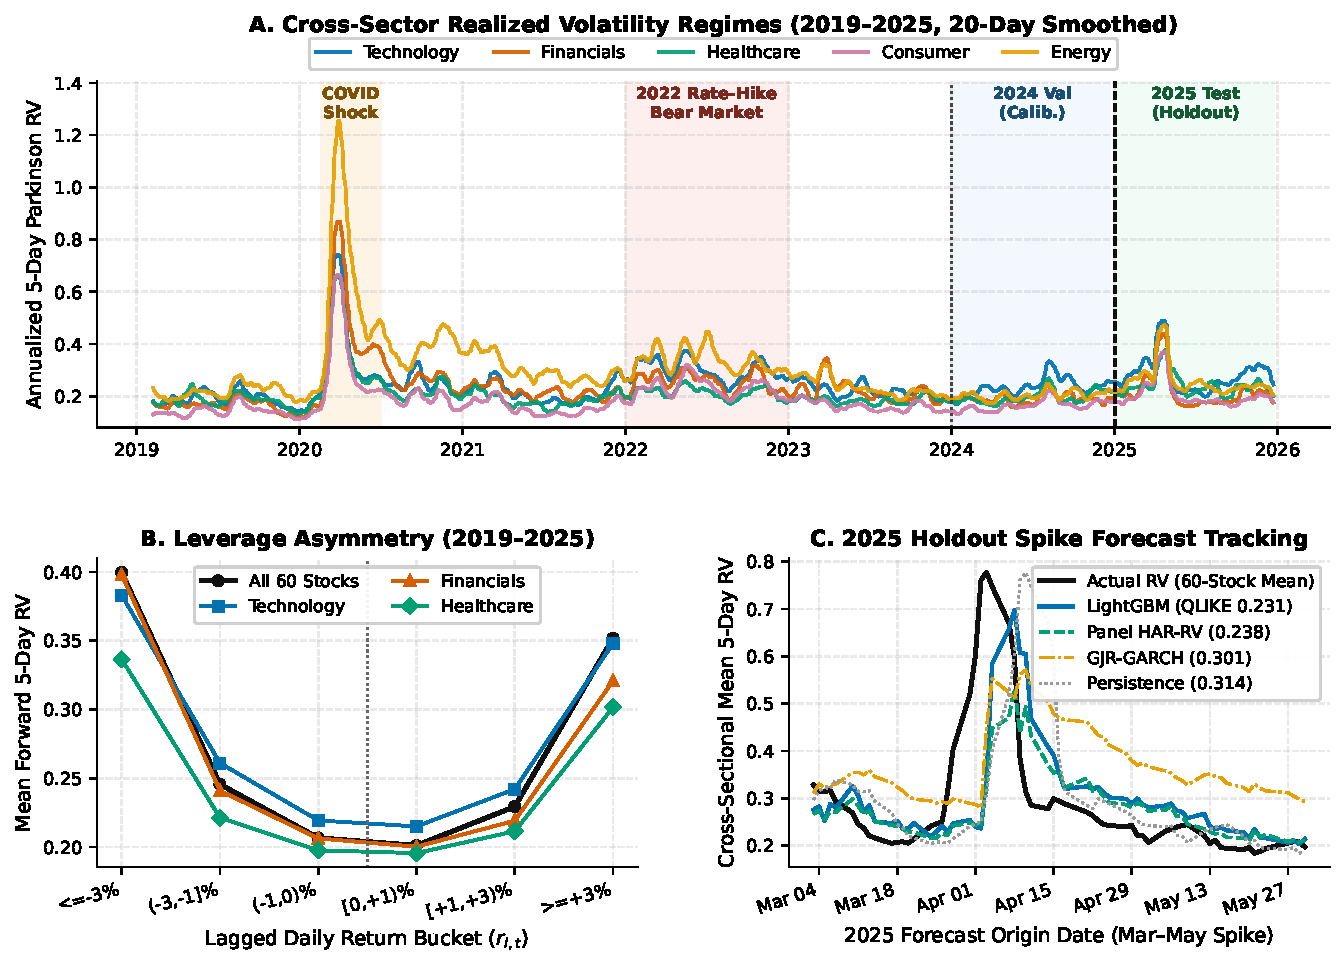
\includegraphics[width=0.86\textwidth]{../outputs/figures/fig1_volatility_regimes_and_forecasts.pdf}
\caption{Cross-sector 2019--2025 volatility regimes (Panel A), lagged return
leverage asymmetry (Panel B), and 2025 holdout forecast tracking during the
March--May volatility spike (Panel C).}
\label{fig:regimes_forecasts}
\end{figure}

\begin{table}[!t]
\centering
\caption{Summary of H1 Stock-FE Extended Panel HAR-RV Confirmatory Tests (2019--2025, $N=104{,}040$, Bartlett Driscoll--Kraay SE with $L=7$) and H2 Single-Shot 2025 Holdout Forecasting Performance ($N=14{,}700$, 245 scorable days, 5-day date-block bootstrap $B=1{,}000$ 95\% CIs, and $h=5$ HLN-DM Holm-adjusted $p$-values vs.\ LightGBM).}
\label{tab:main_summary}
\scriptsize
\setlength{\tabcolsep}{3.5pt}
\renewcommand{\arraystretch}{1.12}
\begin{tabular}{lcccccc}
\toprule
\multicolumn{7}{l}{\textbf{Panel A: H1 Confirmatory Associational Family (Within $R^2 = 0.4736$, Healthcare Reference)}} \\
\midrule
Confirmatory Hypothesis & Estimate / $\chi^2$ & 95\% CI / $F$ & Raw $p$ & Holm $p$ & Sig. & Sample \\
\midrule
Leverage AME (neg\_ret\_1d) & -1.4458 & [-2.0529, -0.8386] & <0.0001 & <0.0001 & Yes & 104,040 \\
VIX AME (per +1 pt) & +0.0141 & [+0.0109, +0.0173] & <0.0001 & <0.0001 & Yes & 104,040 \\
Tech x neg\_ret\_1d vs Health. & -0.6479 & [-1.3868, +0.0910] & 0.086 & 0.171 & No & 104,040 \\
Tech x VIX vs Health. & +0.0009 & [-0.0011, +0.0029] & 0.380 & 0.380 & No & 104,040 \\
Joint 5-Sector Wald (df=8) & 84.84 & F=10.60 & <0.0001 & <0.0001 & Yes & 104,040 \\
\midrule
\multicolumn{7}{l}{\textbf{Panel B: H2 2025 Holdout Test Performance (Base Tail Rate = 8.62\%, 300/300 GJR-GARCH Converged)}} \\
\midrule
Model & QLIKE [95\% CI] & RMSE & PR-AUC [95\% CI] & Brier & ECE (Pre) & DM Holm $p$ (Q/B) \\
\midrule
Persistence (RV\_w / Base) & 0.3144 [0.213,0.484] & 0.1196 & 0.0721 [0.051,0.104] & 0.0788 & 0.0023 & <0.0001 / 0.047 \\
GJR-GARCH(1,1) Per-Stock & 0.3007 [0.241,0.386] & 0.1362 & 0.1271 [0.098,0.169] & 0.0796 & 0.0264 & 0.021 / 0.123 \\
Panel HAR-RV (+ Logistic) & 0.2383 [0.158,0.380] & 0.0957 & 0.1422 [0.104,0.191] & 0.0774 & 0.0070 & 0.134 / 0.716 \\
\textbf{Global LightGBM (Cal.)} & 0.2306 [0.154,0.372] & 0.0951 & 0.1231 [0.083,0.177] & 0.0773 & 0.0102 (0.380) & Ref. \\
\bottomrule
\end{tabular}
\end{table}


\textbf{H2 Single-Shot 2025 Holdout Performance and TreeSHAP Audit.} On 2025
volatility forecasting (Table~\ref{tab:main_summary}, Panel B;
Figure~\ref{fig:regimes_forecasts}C), Global LightGBM achieves the lowest
overall QLIKE (0.2306) and RMSE (0.0951), significantly
outperforming Persistence (QLIKE 0.3144, Holm $p < 0.0001$) and
per-stock GJR-GARCH(1,1) (0.3007, Holm $p = 0.0207$),
and showing its largest QLIKE reduction in Technology (0.2862 vs.\
Panel HAR-RV 0.3369), while full-universe QLIKE vs.\ Panel HAR-RV
(0.2383) is directionally favorable but not statistically
distinguishable (Holm $p = 0.134$). For downside tail-risk
classification, applying the frozen 2024-Val \texttt{isotonic}
calibrator cuts LightGBM's 2025 ECE by 97.3\%
(0.3804 $\to$ 0.0102) and achieves the lowest overall
Brier score (0.0773, Holm $p = 0.0470$ vs.\ Persistence;
Figure~\ref{fig:shap_cal}B). Yet regularized Logistic HAR-RV achieves higher
2025 PR-AUC (0.1422 vs.\ LightGBM 0.1231), especially on
Form 8-K Item 2.02 earnings days (0.2861 vs.\
0.0948). Train-background TreeSHAP (Figure~\ref{fig:shap_cal}A;
additivity error $< 10^{-7}$, positive class 1 verified) reveals that LightGBM
tail-risk probability behavior concentrates on \texttt{rv\_m}
(24.4\%), \texttt{vix\_close} (11.9\%),
and yield-curve slope \texttt{t10y2y}, with amplified attribution magnitudes
under High-VIX regimes.

\begin{figure}[!b]
\centering
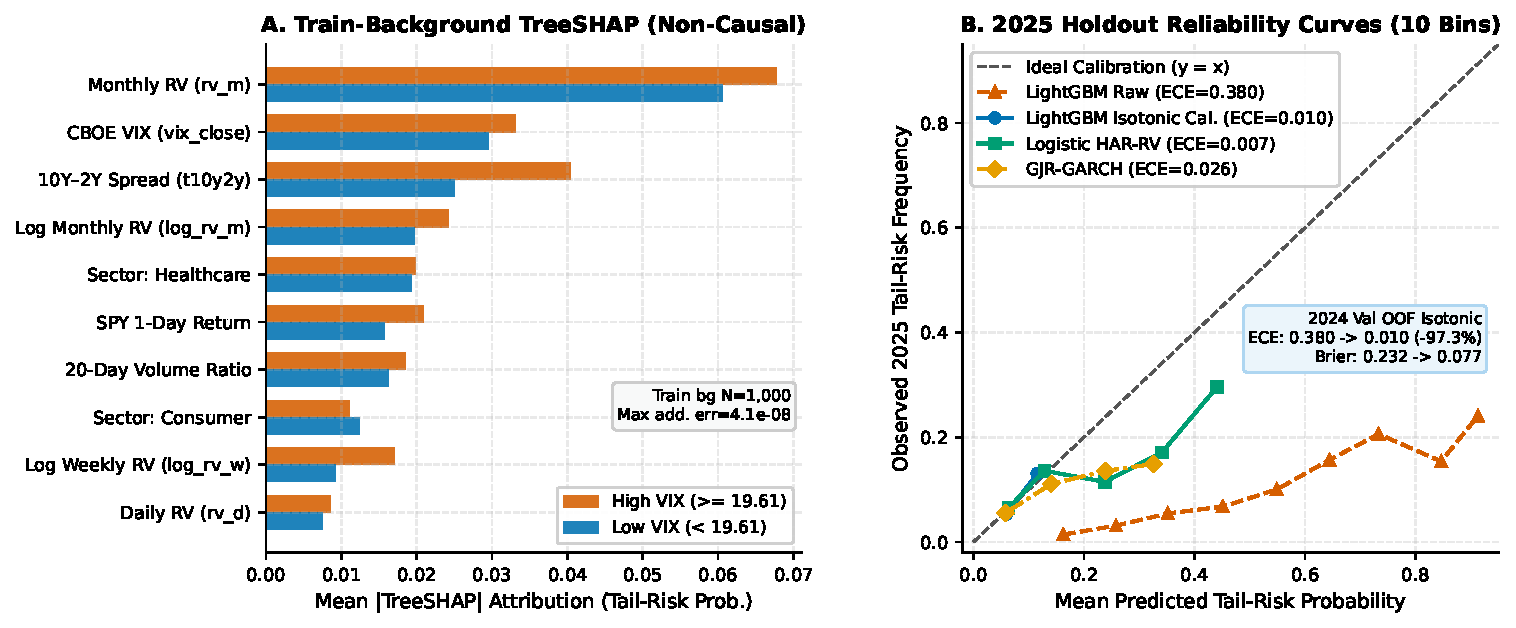
\includegraphics[width=0.84\textwidth]{../outputs/figures/fig2_shap_and_calibration.pdf}
\caption{Train-background TreeSHAP attributions for LightGBM tail-risk model
behavior split by VIX regime (Panel A, strictly non-causal) and 2025 holdout
calibration reliability curves (Panel B).}
\label{fig:shap_cal}
\end{figure}

\section{Discussion, Limitations, and Phase B Outlook}

Our findings yield three practical methodological lessons. First, accounting for
contemporaneous cross-stock correlation via Driscoll--Kraay SEs expands standard
errors by 3.6--4.7$\times$ relative to entity-clustered Newey--West SEs,
preventing false-positive claims on pairwise sector interactions. Second,
class-weighted tree models require out-of-sample post-hoc calibration before
probabilities can be interpreted as risks (cutting ECE by
97.3\%), yet piecewise-constant isotonic steps introduce
upper-tail ties that can compress ranking granularity (PR-AUC) relative to
smooth linear logits on sparse earnings days. Third, all models lag abrupt
overnight macro shocks (such as the April 2025 tariff gap) and binary earnings
jumps because Phase A relies solely on daily OHLCV, macro indicators, and filing
counts.

\textbf{Key Limitations and Scope Boundary.} Our fixed 60-stock
large-cap universe introduces survivorship bias relative to delisted small-caps;
daily Parkinson range volatility contains measurement error compared with
intraday high-frequency RV; and SEC EDGAR filings capture authoritative
corporate disclosures rather than continuous analyst commentary or social media.
These results represent associational and predictive risk benchmarks for CS482
coursework only and \textbf{do not constitute investment advice}.

\textbf{Phase B Extension (Frozen Handoff Ready).} With Phase A data, purged
splits, and 6,822 pre-close event-anchored text rows
cryptographically frozen (\texttt{events\_text\_phase\_b.parquet}), Phase B
will evaluate single-A100 4-bit QLoRA fine-tuning of 27B--32B open financial
LLMs against \texttt{FinBERT} (110M) and price-only Phase A models on the
identical 2025 holdout test set, directly testing H3 on earnings and
material-event days.

% =========================================================================
% EXCLUDED BACK MATTER (References, Contribution Statement, AI Declaration)
% =========================================================================
\clearpage
\bibliographystyle{plainnat}
\bibliography{references}

\clearpage
\section*{Separate Contribution Statement}
\begin{itemize}\setlength{\itemsep}{2pt}
\item \textbf{Member A (Financial Data \& Freeze Lead):} Designed the pre-2019
60-stock universe, built Yahoo/FRED/paginated SEC EDGAR ingestion with
\texttt{BLK}/\texttt{XOM} predecessor CIK linkages, enforced DST-aware
16:00/13:00 ET cutoffs and purged splits, froze \texttt{FREEZE\_MANIFEST.json},
and produced Figure~1.
\item \textbf{Member B (Financial Econometrics Lead):} Implemented cross-cycle
EDA, Stock-FE extended Panel HAR-RV with Bartlett Driscoll--Kraay SE and
Holm-adjusted confirmatory tests, per-stock GJR-GARCH(1,1) convergence audits,
and $h=5$ HLN-DM evaluation.
\item \textbf{Member C (Machine Learning \& Explainability Lead):} Built the
quarterly expanding Global LightGBM pipeline, 2024-Val out-of-fold probability
calibration, Train-background exact TreeSHAP additivity audits, Table~1, and
Figure~2.
\item \textbf{Member D / All Members (Integration, Verification \& Phase B
Prep):} Audited numeric claim traceability against frozen artifacts
(\texttt{phase\_a\_audit.md}), verified formatting and
non-causal/non-investment boundaries, and prepared the frozen Phase B handoff.
\end{itemize}

\section*{AI Usage Declaration \& Academic Integrity}
AI coding and research assistants were used during project planning, code
implementation, test-driven debugging, LaTeX formatting, and prose polishing,
guided by the procedural research guardrails of \citet{kassis2026skills}. All
external data downloads, SHA-256 freeze manifests, econometric standard errors
(cross-checked against \texttt{statsmodels}), 300/300 GJR-GARCH fits,
bootstrap CIs, HLN-DM statistics, TreeSHAP additivity checks ($< 10^{-7}$),
and report numbers were independently executed and verified via deterministic
offline Python scripts (\texttt{uv run python scripts/run\_phase\_a.py
-{}-skip-download}) and automated pytest suites. No fabricated data,
references, or unverified AI outputs appear in this report.

\end{document}
